% !TeX root = ../main.tex
% -*- coding: utf-8 -*-

\chapter{研究基础与现状}
本章首先介绍了纠错性软件维护的相关工作,包括缺陷定位和缺陷预测两个方面;然后介绍了完善性软件维护的研究基
础,主要包括软件质量和代码坏味的关系、软件重构原理和软件重构类型以及软件重构机会推荐方法等。
\section{纠错性软件维护}
纠错性软件维护是提高软件正确性的重要手段,本节主要介绍缺陷定位的相关研究工作,并简单介绍其它纠错性软
件维护,如缺陷预测等。

\subsection{缺陷定位}
软件缺陷是导致软件系统行为失效的主要原因,对软件缺陷的查找和定位是消除软件缺陷的首要步骤。为了帮助软
件维护人员尽可能早地发现缺陷,很多研究致力于提出各种缺陷定位技术来提高纠错性软件维护的效率。当前流行
的缺陷定位技术主要通过覆盖分析、程序切片、依赖分析、程序不变量等方法对缺陷相关代码进行定位。

\subsubsection{基于覆盖分析的缺陷定位方法}
基于覆盖分析的缺陷定位方法是一种轻量级的缺陷定位方法,其流程通常是首先收集程序执行过程中对语句、分
支、谓词等程序元素的覆盖信息,然后利用特定的可疑度计算公式计算代码的可疑度,最后通过优先检查具有较高
可疑度的代码进行缺陷定位。由于基于覆盖分析的缺陷定位方法通常只需要统计测试用例的执行覆盖信息,而不需要
对源代码进行建模,因此计算成本较低,适用于大规模软件系统。

基于覆盖分析的缺陷定位方法在定位缺陷时的流程大致相似,不同方法的主要区别在于可疑度计算方式的不同。目
前,研究者对于可疑度度量公式进行了大量的研究。表~\ref{fig:susp}中列举了六种影响较大的可疑度计算公
式,为了表达更清楚,统一使用以下变量表示对应测试用例的数量:
\begin{itemize}
  \item $a_{00}$表示测试用例被成功执行但未覆盖某个程序元素;
  \item $a_{01}$表示测试用例执行失效且未覆盖某个程序元素;
  \item $a_{10}$表示测试用例被成功执行且覆盖某个程序元素;
  \item $a_{11}$表示测试用例执行失效且覆盖了某个程序元素。
\end{itemize}

Jones等人~\cite{jones2005empirical}等人首次提出基于覆盖分析的缺陷定位方法Tarantula,该方法的核心思想
是被失效用例执行越多、成功用例执行越少的代码可疑度越高~\cite{jones2005empirical},通过为每个语句计算
可疑度,并将可疑度通过可视化的方式展现出来,该方法能够有效定位缺陷代码。基于类似的思想,Wong等人
~\cite{wong2008crosstab}提出基于交叉表的方法计算代码可疑度,该方法通过计算相同程序元素被失效执行和成
功执行的相差次数来计算可疑度。

表~\ref{fig:susp}中的Ochiai公式最早在生物学中作为基因相似度的度量公式被提出,Abreu等人
~\cite{abreu2007accuracy}将其运用到缺陷定位中,通过实验证明Ochiai公式的定位效率优于Tarantula公式。同
时,受聚类分析启发,Abreu等人~\cite{abreu2007accuracy}提出使用Jaccard相似度系数来度量程序代码的可疑
度。同样最早出现在生物学中,Wong等人~\cite{wong2014dstar}对Kulczynski公式
~\cite{willett2003similarity}进行改进,通过捕捉失效用例的相似性来进行缺陷定位。

Naish等人~\cite{naish2011model}对比了36种基于覆盖分析的缺陷定位方法,根据实验结果将基于覆盖分析的缺
陷定位方法根据可疑度计算公式分为等价类,每类的计算公式在性能上等价,并得到Optimal排序方法较其它方法
表现更好的结论。

\begin{center}
\zihaowu
\tablecaption{经典可疑度计算公式}\label{fig:susp}
\begin{tabular}{cc}
\toprule
覆盖分析法 & 可疑度计算公式 \\ \midrule
Tarantula & $\frac{\frac{a_{11}}{a_{11}+a_{01}}}{\frac{a_{11}}{a_{11}+a_{01}}+\frac{a_{10}}{a_{10}+a_{00}}}$\\ 
Jaccard & $susp = \frac{a_{11}}{a_{11}+a_{01}+a_{10}}$\\ 
Ochiai & $susp = \frac{a_{11}}{\sqrt{(a_{11}+a_{01})\times(a_{11}+a_{10})}}$\\
Ochiai2 & $susp = \frac{a_{11}a_{10}}{\sqrt{(a_{11}+a_{10})\times (a_{00}+a_{10})\times (a_{11}+a_{01})\times (a_{01}+a_{00})}}$\\ 
Wong & $susp = a_{11}-a_{10}$\\
DStar & $susp = \frac{a_{11}^{star}}{a_{10}+a_{01}}$\\ 
Naish2 & $susp = a_{11}-\frac{a_{10}}{a_{10}+a_{00}+1}$ \\
Optimal & $susp = \begin{cases}
  -1, & \text{ if } a_{01}>0 \\ 
  a_{00}, & \text{ elsewise }  
  \end{cases}$\\ 
  \bottomrule
\end{tabular}
\end{center}

Santelices等人~\cite{santelices2009lightweight}通过实验评估了不同覆盖特征对缺陷定位效率的影响,分别
比较了语句、分支和定义使用对三种覆盖特征,发现这三种覆盖特征分别对特定类型的缺陷有较好的定位效果。在
此基础上,他们提出结合方法来使缺陷定位技术对所有类型的缺陷都具有较好的定位效果,通过分别计算三种覆盖
特征下的可疑度并计算可疑度平均值,得到综合效果最好的缺陷定位方法。

不同于以上基于覆盖分析的缺陷定位方法,Renieres~\cite{renieres2003fault}提出了基于并集和交集的方法来定
位缺陷,该方法不需要计算可疑度公式,而是分别统计被失效用例覆盖但未被成功用例覆盖的语句集合和被所有成
功用例覆盖但未被失效用例覆盖的语句集合来定位缺陷。

\subsubsection{基于程序切片的缺陷定位方法}
程序切片是一种重要的程序分析技术,该技术通过分析程序的数据流和控制流依赖关系来了解程序。Weiser等人
~\cite{weiser1981program}最早提出静态程序切片技术,通过切片准则计算出语句集合。由于静态切片中包含大
量与程序失效无关的语句。为了缩小可疑代码的范围,Korel等人~\cite{korel1988dynamic}提出动态切片的方
法,计算在特定输入下与程序失效有关的语句集合,从而缩小可疑代码的范围。根据切片的方向不同,动态切片方
法可分为前向和后向动态切片~\cite{korel1994forward},分别计算影响某个变量值的语句集合和被某个变量值所
影响的语句集合。

虽然动态切片相比较静态切片所得到的可疑代码范围较小,但面对大规模软件系统时,动态切片计算得到的语句集
合规模仍然很大。为了减小动态切片的规模,Zhang等人~\cite{zhang2007locating}提出了一种基于多点切片的缺
陷定位方法,从关键谓词、错误值和导致错误值的输入三点计算切片,从而缩小可疑代码范围。Hofer等人
~\cite{hofer2012combining}引入了基于约束的方法,通过约束求解缩小动态切片的语句集合。Wong等人
~\cite{wong2004execution}将动态切片与数据依赖相结合,通过将成功用例和失效用例的切片相减来得到削片,
通过查找削片中语句的数据依赖来定位缺陷。Gupta等人~\cite{gupta2005locating}提出了基于动态砍片的缺陷定
位技术,通过Delta调试减小能够导致程序行为失效的输入范围,并计算该输入范围内的前向切片集合和导致失效
输出的后向切片集合,通过求这两个动态切片集合的交集,得到动态砍片来定位缺陷。

虽然基于程序切片的方法能够有效地减小缺陷的搜索范围,但由于动态切片的计算复杂度较高,这类方法通常被认
为是一种重量级的方法。

\subsubsection{基于依赖分析的缺陷定位方法}

为了分析语句之间的依赖关系,Baah等人~\cite{baah2010probabilistic}提出了概率程序依赖图模型,在程序依
赖图的基础上增加了表示语句的结点和表示控制依赖和数据依赖的边,通过执行测试用例,得到与执行有关的状态
集合来记录程序的内部行为,通过对缺陷相关程序行为的不确定性进行概率分析来定位缺陷。Zhang等人
~\cite{zhang2009capturing}在程序控制流图的基础上提出了概率模型,从程序中抽取控制流图,通过分析控制流
图中程序状态的感染趋势计算每个节点的可疑度。Gong等人~\cite{gong2015state}提出了状态依赖概率模型,通
过路径分析得到在特定状态下代码的控制依赖关系,通过比较成功用例和失效用例之间状态的不同来定位缺陷。

\subsection{数据驱动的纠错性软件维护}

\subsubsection{数据驱动的缺陷定位}
由于程序的失效行为与程序缺陷之间存在关联性,因此部分研究者提出基于关联规则的方法来定位缺陷。Denmat等
人~\cite{denmat2005data}提出了基于关联规则的缺陷定位方法,通过挖掘失效用例的执行轨迹,使用关联规则中
的置信度与支持度来筛选缺陷相关语句。赵磊等人~\cite{zl}认为高可疑代码与缺陷性相关代码的执行路径存在较
强的关联,因此通过对测试用例的执行路径进行分析和频繁集求解,挖掘高可疑代码的关联代码,然后利用传统的
基于覆盖分析的可疑度计算公式计算代码的可疑度来进行缺陷定位。基于类似的思想,Cheng等人
~\cite{cheng2009identifying}将测试用例的执行路径表示为图,通过提取可判别子图比较成功用例和失效用例之
间的差异,从而缩小缺陷搜寻范围。除关联分析外,Brun等人~\cite{brun2004finding}提出基于支持向量机的缺
陷定位方法,通过动态不变量检测生成程序的不变量表达式,通过机器学习模型对不变式进行分类,通过预测不变
式可能导致缺陷的概率来定位缺陷相关代码。张云乾等人~\cite{malcov2013}认为缺陷定位技术的准确性和缺陷类
型有关,因此提出使用马尔科夫模型预测缺陷类型,然后选用有针对性的缺陷定位技术进行缺陷定位。

除此以外,部分学者使用聚类分析将失效用例进行聚类~\cite{jones2007debugging, zheng2006statistical},对
每类失效用例采用单缺陷的方法进行处理。基于聚类分析的方法,其核心思想是由相同缺陷引起的失效用例其程序
行为相似,具有相似的覆盖信息。这种方法虽然在一定程度上提高了多缺陷的定位准确率,但是依赖聚类分析的准
确性,很难完全避免多缺陷之间的相互影响。何加浪等人~\cite{neural2013}使用神经网络学习输入和缺陷之间的
关系,计算代码的各个位置与每个缺陷之间的相关性来定位缺陷。

\subsubsection{数据驱动的缺陷预测}

目前数据挖掘在缺陷预测上的应用较为广泛,很多研究者提出了各种缺陷相关软件度量以及机器学习模型来进行缺
陷预测。Menzies等人~\cite{menzies2007data}使用朴素贝叶斯模型进行缺陷预测,并提出在预处理阶段,使用对
数操作可以提升缺陷预测能力。Elish等人~\cite{elish2008predicting}通过在NASA数据集上的对比实验,比较了
支持向量机、逻辑斯特回归、朴素贝叶斯、决策树和神经网络在缺陷预测任务上的表现,得到支持向量机是用于缺
陷预测的最优模型。

为了解决基于机器学习的缺陷预测模型中数据不平衡的问题,Drown等人~\cite{drown2009evolutionary}提出了基
于遗传算法的缺陷预测模型,利用遗传算法中的指标优化采样过程。Khoshgoftaar等人
~\cite{khoshgoftaar2010attribute}提出结合特征选择和采样的模型来进行缺陷预测。Pelayo等人
~\cite{pelayo2012evaluating}通过对下采样和上采样进行对比实验,认为下采样的性能更好,并提出可以将两种
采样方法相结合来提高缺陷预测的准确性。

\section{完善性软件维护}

\subsection{代码坏味}
代码坏味是软件系统中出现``坏代码''的信号,通常被研究者认为软件系统需要进行重构的信号。Fowler等人提出
了22种软件结构作为代码坏味的表现,并认为这些代码坏味可以帮助软件维护人员决定软件是否需要被重构
~\cite{fowler1999refactoring}。Palomba等人~\cite{palomba2015mining}提出通过挖掘软件系统的历史行为来
检测代码坏味。Fowler等人提出了72代码重构操作,在保持程序外在行为的一致性的同时,改进程序内部的设计结
构~\cite{fowler1999refactoring}。在表~\ref{fig:badsmell}中我们列举了其中十种经典的代码坏味,以及可能
解决这些代码坏味的软件重构操作。

\begin{center}
\zihaowu
\tablecaption{常见代码坏味}\label{fig:badsmell}
\begin{tabular}{lll}
\toprule
 代码坏味 & 软件重构操作 & 重构目标\\ \midrule
 代码重复 & 函数提炼、函数上移、类提炼 & 提取公共代码\\ 
 函数过长 & 函数提炼 & 拆分函数\\ 
 类过大 & 类提炼 & 拆分类\\ 
 参数过多 & 引入参数对象、函数替代参数 & 减少参数\\ 
 发散式变化& 类提炼 & 将全部变化提取到新类\\ 
 霰弹式改动& 函数移动、类内联 & 将全部修改合并为同类\\ 
 依恋情节& 函数提炼、函数移动 & 移动依恋代码\\ 
 数据泥团& 类提炼、引入参数对象 & 简化数据\\ 
 基本类型偏执& 对象替换数据 & 简化类型 \\ 
 Switch语句 & 函数提炼、函数移动 & 减少Switch语句\\ 
\bottomrule
\end{tabular}
\end{center}

值得注意的是,每一种代码坏味可以被一种或多种软件重构操作所解决。如表~\ref{fig:badsmell}中的代码重
复,在很多情况下可以通过函数提炼(Extract Method)提取重复的代码结构作为一个新的函数被调用;当重复代
码出现在两个兄弟子类时,可以分别在这两个子类中进行函数提炼,然后将该函数上移(Pull Up Method)到这两
个子类的父类中;当重复代码出现在两个不相干的类中时,可以将重复代码提取为一个新类(Extract Class),
在原来的两个类中调用这个新类。可以看出,即使针对同一代码坏味,在不同的情况下软件维护人员需要选择不同
的重构操作,甚至是一系列重构操作的叠加。不同的软件重构操作通常会对软件系统有不一样的影响,因此软件维
护人员需要谨慎选择软件重构的类型。

同时,代码坏味不完全是相互独立的,有一些代码坏味是相关联的,因此可以被相同的软件重构操作所解决。例如
代码重复可能会导致函数过长或者类过大,此时如果使用函数提炼或类提炼,既解决了代码重复的问题,同时也解
决了函数过长或者类过大的问题。同样,依恋情节通常发生在某个函数对某个类的兴趣远高于其所在的类,此时会
导致该函数频繁的访问该类,可能导致函数过长、类过大、参数过多以及发散式变化(容易受到该类的影响)等代
码坏味。通过将部分依恋代码提炼成新的函数,并移动到其频繁访问的类(Move Method),可以让大部分问题得
到改善。由于部分代码坏味能够被相同的软件重构类型所解决,因此通过优化软件重构的顺序通常可以减少还需进
行的软件重构数量。

有一些代码坏味是互斥的,因此它们所对应的软件重构操作也是互为逆向操作。如表~\ref{fig:badsmell}中的类
过大和霰弹式改动是两个互斥的代码坏味。当我们用类提炼将大类拆分成多个小类时,虽然每个类的规模变小,但
容易引发霰弹式改动的问题,即原来在同一个大类中的多个小类由于彼此依赖,导致当改动其中一个小问题时,引
发一系列发散的改动,造成软件维护的不便;反之,当我们用类内联(Inline Class)将某个修改所涉及到的修改
都集合到同一个大类中时,虽然解决了霰弹式改动的代码坏味,但此时容易引起类过大的问题。这样逆向的软件重
构操作还有函数提炼和函数内联(Inline Method)、函数上移和函数下移(Pull Down Method)等。因此,如何
针对软件系统选取合适的软件重构操作是软件维护人员需要解决的问题。

虽然代码坏味是软件重构的重要信号,但是软件重构的动机却不完全是为了解决代码坏味。Silva等人
~\cite{silva2016we}调查研究了软件开发人员进行软件重构的动机。调查发现,软件重构主要发生在需求发生改变
的时候,如增加新特性或是修复软件缺陷时,因此软件重构的动机通常与提高软件的易读性、可重用性、易测性等
相关,而不仅仅是针对特定代码坏味的修复。以最常用的软件重构操作--函数提炼为例,调查显示,软件维护人员
进行函数提炼重构的原因较为复杂,包括代码重用、函数分解、加速扩展、重命名内部函数等11种主要原因。其
中,只有函数分解与代码坏味有关,其通常被认为是决代码坏味``函数过长''的方法。由于人工识别软件重构机会
并选择软件重构操作的成本较高,且软件重构的动机具有复杂性和多样性,研究者们提出了很多软件重构推荐技术
来解决该问题,关于软件重构推荐的研究引起了广泛关注。

\subsection{软件重构原理}
软件重构提高软件质量,是降低软件维护成本的重要手段之一。重构这个术语最早由William
Opdyke~\cite{opdyke1992refactoring}在其博士论文中提出的。软件重构技术旨在在不改变软件整体功能的前提
下,改进软件的设计结构,使得新的设计结构提高代码的可维护性,从而提高软件的质量
~\cite{fowler1999refactoring}。因此,软件重构通常只改变软件的外观,比如在传统的结构化设计上以改进其
结构。软件重构不涉及修改软件的语义和功能,而是通过更好的观察软件系统,从而提出对软件系统设计各方面的
改进~\cite{chikofsky1990reverse}。

\begin{figure}
  \centering
  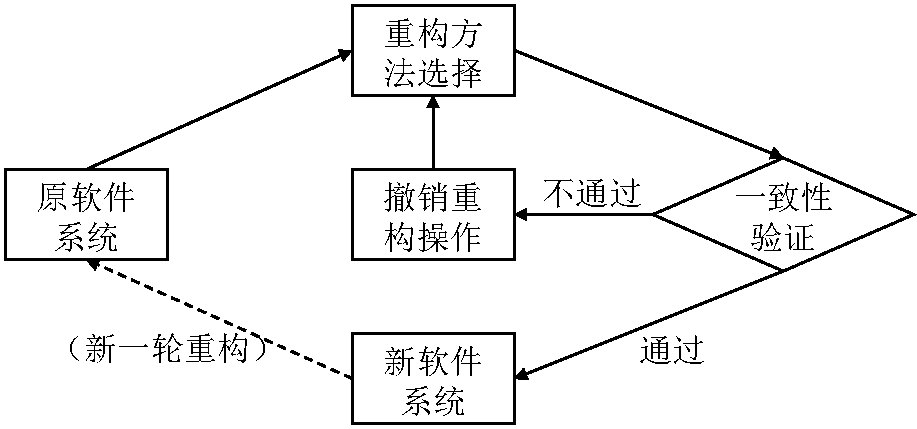
\includegraphics[height=60mm, width=90mm]{refactory.pdf}  
  \caption{\label{fig:refactory}软件重构一般过程}
\end{figure}

软件重构的一般过程是通过迭代转换的方式对软件系统进行转换。图~\ref{fig:refactory}描述了这样的转换过程。针
对原软件系统,每一轮迭代是对软件的一次小规模转换,针对特定代码选择某种重构方法,在实施软件重构操作后
测试其正确性,即测试软件的语义和功能是否与原来的保持一致。若测试通过,则本轮重构完成,软件维护人员可
在新的软件系统上进行新一轮重构。在任何时间一旦测试不通过,则最后一次程序转换撤销,需要重新选择重构方
法,换一种方式进行重构。通过很多轮这样的小规模程序转换,软件重构的过程和细节可以完全被软件维护人员所
掌控,并达到其所预想的效果。这样的迭代过程要求测试过程十分迅速,否则软件维护人员将不得不花费大量的时
间等待测试完成。因此,很多极限编程和其它敏捷软件开发的使用者将这种迭代过程作为软件开发周期的一个重要
组成部分。除此以外,为了减少一致性验证所带来的测试时间成本,部分学者提出使用先置性条件过滤,使得满足
条件的软件重构能保持语义和功能的一致性,从而减少不必要的测试成本。

软件重构是影响软件完善性维护的重要方面。在软件生命周期中,新的需求被不断添加,使得代码的复杂度越来越
高,代码结构逐渐偏离原来的设计,从而导致了扩展软件的难度越来越大。软件重构增加了程序设计的灵活性,通
过改进软件设计,使得软件具备高内聚、低耦合和复杂度低等特点,将复杂代码变简单,从而提高代码的可扩展
性,降低软件的维护成本。完善性软件维护的时机通常与软件系统质量有关。软件质量下降时,软件系统发出需要
重构的信号。最常见的情况是当软件维护人员修补缺陷或添加新功能时,首先要需要做的就是理解代码。当代码可
读性强,容易被理解时,修复软件缺陷和添加新功能的效率更高。相反,当代码复杂度高、不容易被理解时,代码
的质量下降,可维护性也随之降低,此时通常需要对软件进行重构。完善性软件维护可以加速当前和未来对代码的
理解,从而提高软件维护效率。

为了帮助软件维护人员熟悉代码改变的意图,更好地了解软件的演化过程,很多研究者提出软件重构检测方法来检
测重构历史。Robbes等人~\cite{robbes2008spyware}开发了一个工具集Spyware来监视集成开发环境。该工具将软
件开发人员对代码的修改表示为基于语义的修改序列,并将这些重要的修改存储起来,开发者可以通过观察和重放
这些修改来观测到软件重构的发生。

大多数研究者主要通过比较两个软件版本中代码的相似度来检测软件重构。Demeyer等人
~\cite{demeyer2000finding}首次提出通过比较相同软件系统的不同版本来检测软件重构的方法,该方法通过比较
软件度量,如代码行数(LOC)和函数调用个数等,检测是否存在软件重构。Malpohl等人
~\cite{malpohl2003renaming}通过使用diff命令来比较两个函数的相似度,从而推测出函数重命名的重构操作。
Antoniol等人~\cite{antoniol2004automatic}提出了基于向量空间的信息检索方法检测代码重构。Xing等人
~\cite{xing2005umldiff}基于命名和结构相似度,自上之下比较了包、类、接口等程序元素。同样基于相似度原
理,部分研究者将克隆检测器应用于软件重构检测中,将不同版本的函数相对应,从而检测出函数提炼和函数移动
等软件重构操作~\cite{van2003reconstruction,kim2005functions}。Weißgerber等人
~\cite{weissgerber2006identifying}提出将软件仓库通过预处理存储进关系型数据库中,然后将每次提交的代码
修改作为事务创建,从中分析出增加、修改或删除的类、字段和函数,从而得到可能的软件重构操作,最后使用克
隆检测将这些操作排序。

由于软件重构的本质是保持软件的语义不变,改变其内部结构,因此有研究者提出使用基于语义分析的方法检测软
件重构。Dig等人~\cite{dig2006automated}开发了基于Eclipse的插件,其首先通过语义分析函数调用、类型使
用、实例化等关系,然后使用一种迭代的方法自顶而下的检测重构。Fluri等人~\cite{fluri2007change}比较了两
个版本的抽象语法树,计算了基于抽象语法树的修改操作,并将其映射到抽象语法树级别的代码修改上。这种方法
的优点在于识别了语法树级别的原子改变,但是由于其停留在原子改变,而未将多处改变抽象化分析,导致其很难
检测出更抽象级别的软件重构。

由于基于相似度比较的软件重构检测方法,其侧重点在于不同版本的软件系统的比较,导致其所能检测出的软件重
构的类型有限,大多为函数移动、函数重命名等简单的重构类型;而复杂重构类型往往涉及多处修改,因此很难被
基于相似度比较的方法检测到。Taneja等人~\cite{taneja2007automated}开发了一种工具RefacLib,通过句法分
析来检测代码库的不同版本之间可能存在的软件重构操作。Kim等人~\cite{kim2007automatic}提出了一种基于规
则的识别代码修改的方法,发现并总结了代码改变的逻辑规则,通过自动匹配不同软件系统的函数并根据该逻辑规
则检测软件重构。Xing等人~\cite{xing2006refactoring}将32种特定类型的软件重构表示成查询语句,提出了基
于代码改变的查询方法,将不同软件版本在软件设计的改变提取到数据库中,查询满足软件重构规则的重构操作实
例。Prete等人~\cite{prete2010template}提出了基于逻辑的方法来检测软件重构,根据模板逻辑规则将每个重构
类型表示出来,并使用逻辑编程引擎来推测重构实例。他们开发了工具Ref-Finder,从代码结构上分析了63种软件
重构类型所对应的重构前后的改变。


\subsection{软件重构推荐}

研究者们提出了很多面向软件重构的技术和工具,主要可以分为两类:手动和自动化的方法。第一类方法主要通过
开发支持软件重构操作的工具,执行开发者指定的软件重构操作。第二类方法通过自动推荐可以被软件维护人
员直接采用的重构序列来提高软件质量\cite{harman2007pareto, kessentini2011design,
ouni2013maintainability, Silva2014}。这种序列可以是一个完整的重构方案,即软件维护人员必须接受完整的
解决方案;也可以是针对特定重构类型的推荐序列,维护人员可以通过逐步交互的方法来完全控制他们所要应用的
重构,通过有针对性的修复来提高软件质量。

软件重构的一般过程是选定待重构代码,然后选择软件重构操作,在进行重构后对软件的一致性进行检测,确保该
软件重构操作没有改变软件原有的语义和功能。由于软件重构原因和过程的复杂性,导致软件维护人员需要根据自
己对软件系统的理解,不断做出决策,耗费大量的时间和精力成本。尤其是当重构操作涉及到不止一个文件和代码
包时~\cite{liu2013monitor},因此,自动软件重构技术越来越得到研究者们的关注。本节首先介绍软件重构操作
的自动检测技术,然后介绍软件重构推荐的相关技术,包括软件重构机会的识别和推荐,以及软件重构顺序推荐,
最后介绍软件重构的一致性相关研究。


虽然半自动的软件重构过程可以省去不必要的人工操作和验证,但其仍然依赖于程序员对软件系统的理解来做出一
系列适合当前软件系统的决策。为了提高软件重构效率,已经有很多工作致力于软件重构机会的识别和推荐。关于
软件重构机会推荐的工作通常包括两个方面,分别是软件重构机会的识别和软件重构操作推荐。这两个方面分别对
应着软件重构的两个关键步骤:(1)识别选定代码是否存在软件重构机会(2)为选定代码推荐合适的软件重构操
作。通常情况下,只有识别了软件重构机会,才有可能对软件进行重构。而人工识别软件重构机会往往要求软件维
护人员对软件系统的设计和实现有全局的了解,因此对软件维护人员的经验和能力要求较高,尤其是在不用程序分
析工具的情况下,了解软件系统的设计并识别软件重构机会是一个复杂而耗时的过程。值得注意的是,部分研究将
这两个步骤融合在一起,在识别软件重构机会的同时推荐重构操作。例如,当我们对代码进行克隆检测
~\cite{kamiya2002ccfinder}的同时,如果我们检测到了克隆代码,往往使用函数提炼或类提炼等重构将公共代码
提取出来,以便复用。根据主要方法的不同,我们可以将关于软件重构机会推荐的研究分为六类
~\cite{al2015identifying}。

由于软件重构的主要原因之一是改善软件设计、提高软件质量,而软件质量度量通常被认为是衡量软件质量的重要
指标,因此大部分关于软件重构机会推荐的研究,通过软件质量度量评价软件重构机会的优劣。Meananeatra等
~\cite{meananeatra2011using}提出了基于软件可维护性度量的方法来推荐五种软件重构,该方法通过比较重构前
和重构后的软件系统的复杂度、规模和凝聚度,选择能够优化软件质量度量的重构进行实施。Yoshida等人
~\cite{yoshida2012cohesion}建议根据功能将函数体进行拆分来生成函数抽取软件重构机会,并根据内聚度来选择重
构机会。Demeyer等人~\cite{demeyer2000finding}提出了一种软件重构机会的检测方法,通过软件度量包括函数
规模、类规模、继承相关度量等面向对象的软件质量度量来识别重构机会,从而推荐与拆分或合并类有关的软件重
构。Yang等人~\cite{yang2009identifying}提出了针对规模较大的函数利用函数的层次结构将长函数拆分成多个
代码片段作为函数抽取重构机会,并通过函数复杂度来对重构机会进行排序。Charalampidou等人
~\cite{charalampidou2016identifying}通过识别连续的有共同变量的语句来识别函数抽取重构机会,并根据内聚
度评价重构机会。

除了软件质量度量,部分研究者提出基于程序切片的方法来识别和推荐软件重构机会。Maruyama等人
~\cite{maruyama2001automated}首次提出使用程序切片来识别函数抽取重构机会,利用基本块来限制程序切片的
范围,但由于其无法从语法上保证抽取代码段前后程序的行为保持一致,因此其实用性受到了限制。Tsantalis等
人~\cite{tsantalis2011identification}针对给定变量和对象,通过计算程序切片得到所有可能改变变量的值或
对象的状态的可执行切片。通过对程序切片的完全计算,该方法能够对给定的切片要求(如某个特定的变量),在
提取出所有与指定要求相关的代码片段的同时不改变原来的程序行为。

由于软件维护的过程中通常需要不止一次重构,才能达到改善软件设计、提高软件质量的目的,为了提高完善性软
件维护的效率,很多研究者针对如何对软件重构操作进行排序展开了研究。刘辉等人
~\cite{liu2009facilitating}通过代码坏味推荐软件重构顺序,分析了代码坏味之间的关系,以及代码坏味的处
理顺序对软件质量的影响,最后提出了基于代码坏味处理顺序的软件重构顺序推荐。Vidal等人
~\cite{vidal2016approach}根据软件系统的历史和组件重要性来对检测出的代码坏味进行排序,并根据代码坏味
的顺序进行软件重构。Qayum等人~\cite{qayum2009local}提出了基于图的软件重构顺序推荐方法,图中结点表示
软件重构,边表示重构的相互依赖关系,通过蚁群优化方法检测软件重构之间的是否存在依赖或者冲突,从而优化
软件重构顺序。Piveta等人~\cite{piveta2008searching}认为合理的软件重构顺序能够有效减少剩余可重构数
量,因此他们提出了基于确定有限自动机的软件重构顺序推荐方法,通过寻找能够缩短软件重构序列的路径来优化
重构顺序。针对克隆代码,Lee等人~\cite{lee2011automated}提出使用面向对象模型中的属性度量重构前后的软
件质量,从而选择使软价质量度量提升最大的重构序列作为最优序列。
